\subsection{Untersuchung der Filterkurve}

Vor der eigentlichen Untersuchung der Filterkurve wird die Verstärkung berechnet.
Eingestellt war eine 10-fache Verstärkung.
Ohne den Selektivverstärker betrug die Spannung des Synthesizers $\SI{0.6}{\milli\volt}$,
mit diesem $\SI{4.5}{\milli\volt}$.
Das entspricht einer tatsächlichen Verstärkung von $\num{7.5}$.

\begin{table}
  \centering
  \caption{Messdaten zur Bestimmung der Filterkurve.}
  \label{tab:filterkurve}
  \begin{tabular}{S[table-format=2.2] S[table-format=3.1]}
  \toprule
  $\nu \mathbin{/} \si{\kilo\hertz}$ &
  $U_A \mathbin{/} \si{\milli\volt}$ \\
  \midrule
  % \expandableinput{build/table_filterkurve.tex}
  20    & 92.5  \\
  21    & 87.5  \\
  22    & 102.0 \\
  23    & 118.0 \\
  24    & 138.0 \\
  25    & 162.0 \\
  26    & 194.0 \\
  27    & 234.0 \\
  28    & 291.0 \\
  29    & 320.0 \\
  30    & 440.0 \\
  31    & 625.0 \\
  31.5  & 750.0 \\
  32    & 870.0 \\
  32.25 & 918.0 \\
  32.5  & 948.0 \\
  33    & 937.0 \\
  33.25 & 900.5 \\
  33.5  & 850.0 \\
  34    & 735.0 \\
  34.5  & 625.0 \\
  35    & 532.0 \\
  36    & 398.0 \\
  37    & 310.0 \\
  38    & 247.0 \\
  39    & 200.0 \\
  40    & 165.0 \\
  \bottomrule
  \end{tabular}
\end{table}

Um die Filterkurve charakterisieren zu können,
wurde aus den aufgenommenen Daten,
die in \autoref{tab:filterkurve} dargestellt sind,
mithilfe von \textit{scipy} ein Fit an die Lorentzkurve
\begin{equation*}
  f(\nu) = \frac{a}{(\nu^2-\nu_0^2)^2 + \gamma^2 \nu_0^2}
\end{equation*}
berechnet.

Die resultierenden Fit-Parameter sind :
\begin{align*}
  \nu_0 &= \SI{32.793(61)}{\kilo\hertz} \\
  a &= \SI{33153365(1869152)}{\kilo\hertz\tothe{4}\milli\volt} \\
  \gamma &= \SI{-5.806(188)}{\kilo\hertz} \; .
\intertext{Durch Umstellen und Einsetzen ergibt sich weiterhin}
  \nu_- &= \SI{30.868}{\kilo\hertz} \\
  \nu_+ &= \SI{34.611}{\kilo\hertz} \; .
\end{align*}

Der Fit-Parameter $\nu_0$ liefert direkt die Durchlassfrequenz $\nu_0 = \SI{32.793(61)}{\kilo\hertz}$.

\begin{figure}
  \centering
  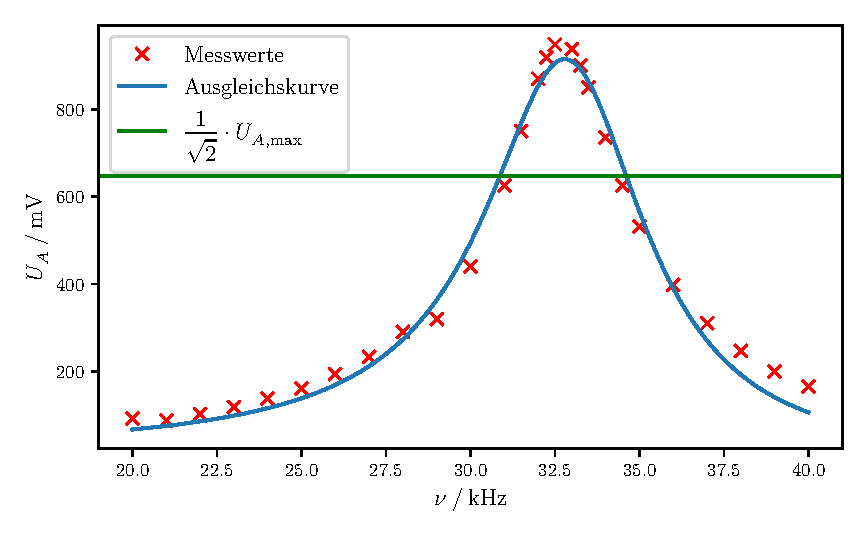
\includegraphics[width=\textwidth]{build/plot_filterkurve.pdf}
  \caption{Filterkurve.}
  \label{fig:plot_filterkurve}
\end{figure}

Die Güte berechnet sich nach
\autoref{eqn:güte}
zu {
\label{misc:güte}
$8.7611 \pm 0.0164$
}.
% Wow, das ist klein.
% 70 (gemessen) / 100 (Geräteangabe) → Renameus
% 100.57 → aknierim
